% Minh chứng CI – nguồn: docs/process/sprint-1.md mục 4
\subsubsection*{Minh chứng pipeline}

\begin{longtable}{|p{3.0cm}|p{1.5cm}|p{6.3cm}|p{3.8cm}|}
\caption{Các lần chạy CI của Sprint 1}\label{tab:ci-runs}\\
\hline
\thead \textbf{Lần chạy} & \textbf{Commit} & \textbf{Kết quả} & \textbf{Link} \\ \hline
\endfirsthead
\hline
\thead \textbf{Lần chạy} & \textbf{Commit} & \textbf{Kết quả} & \textbf{Link} \\ \hline
\endhead
PR \#30 -- lần 1 & \code{96a0197} & \textbf{Cancelled}: commit mới được push nên workflow tự hủy lượt cũ & \href{https://github.com/dangpham-work/CupPulse/actions/runs/41408066493}{run 41408066493} \\ \hline
PR \#30 -- lần 2 & \code{cd3f53d} & \textbf{Success}: quality 1m 0s, integration 43s, docker 1m 53s & \href{https://github.com/dangpham-work/CupPulse/actions/runs/41408203576}{run 41408203576}, \href{https://github.com/dangpham-work/CupPulse/pull/30}{PR \#30} \\ \hline
PR \#31 (minh chứng lỗi) & \code{89d5753} & \textbf{Failure} ở bước \textbf{Lint}: biến không dùng; Typecheck, Unit Test, Build bị bỏ qua; job Docker cũng đỏ vì \code{next build} chạy ESLint & \href{https://github.com/dangpham-work/CupPulse/actions/runs/41408237890}{run 41408237890}, \href{https://github.com/dangpham-work/CupPulse/pull/31}{PR \#31} (đóng, không merge) \\ \hline
\end{longtable}

\begin{figure}[H]
\centering
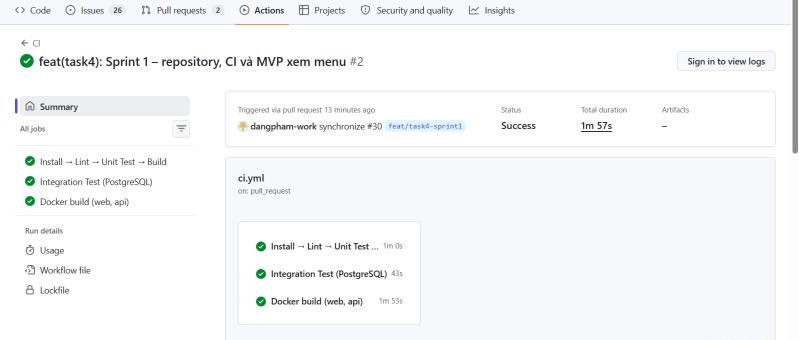
\includegraphics[width=0.9\textwidth]{figures/ci-pass.png}
\caption{CI của PR \#30 thành công: ba job xanh}\label{fig:ci-pass}
\end{figure}

\begin{figure}[H]
\centering
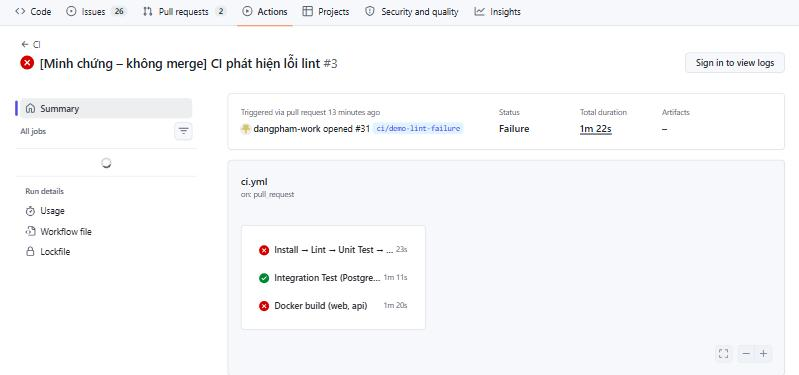
\includegraphics[width=0.9\textwidth]{figures/ci-fail.png}
\caption{CI của PR \#31 phát hiện lỗi lint: job chất lượng và job Docker đỏ}\label{fig:ci-fail}
\end{figure}

Trích log bước Lint của run 41408237890:

\begin{lstlisting}[basicstyle=\ttfamily\scriptsize,frame=single]
apps/web lint:   27:7  error  'unusedForCiDemo' is assigned a value but never used
                 @typescript-eslint/no-unused-vars
apps/web lint: x 1 problem (1 error, 0 warnings)
\end{lstlisting}

\textbf{Sự cố trong Sprint.} Mẫu \code{.gitignore} Python có dòng \code{lib/} làm
\code{apps/web/src/lib/api.ts} không được commit ở lần push đầu (máy local vẫn build được vì tệp có trên đĩa). Lỗi
được phát hiện khi chuẩn bị nhánh minh chứng, trước khi lượt CI đầu chạy xong, và được sửa ở commit \code{cd3f53d}.
Bài học: CI trên máy sạch là nơi kiểm chứng repository đầy đủ, nên luôn chờ CI xanh trước khi merge.
